\documentclass{article}
\usepackage[utf8]{inputenc}
\usepackage{graphicx}
\usepackage{subcaption}
\usepackage{grffile}
\usepackage{amsmath}
\usepackage{bm}


\title{Numerics for Articles 1 and 2}
\author{Yuval Kochavi}
\date{December 2025 - January 2026}

\begin{document}

\maketitle

\section{Foam Simulation - simple HR comparison}
First, the key difference in this code is that $T_{\text{bath}}$ varies in time, and the material can be switched between foam and gold. The $T_D$ values (i.e., $T_{\text{bath}}$ at each time in ns) were sampled from the green curve in Cohen\&Heizler (2018, Fig.~3).

The implementation required several iterations to achieve stable behavior. The foam parameters were taken from the Back et al. experiment, as described in the paper. A major issue in this simulation is that the results are very sensitive to the exact parameter values, especially the opacity parameters. After many hours of debugging, Shay suggested changing the harmonic averaging in the \texttt{D\_face} calculation to arithmetic averaging, which made the simulation much more stable. With harmonic averaging, the foam heat-front position was off by about three orders of magnitude (roughly $10^{-4}\,\mathrm{m}$). After this change, I ran the simulation and compared it to the simple HR 1D model using $T_s=T_D$.
% \begin{figure}[h!]
%     \centering
%     \includegraphics[width=1\linewidth]{figures_article1/foam_HR_comparison(nonmarshak).png}
%     \caption{Comparison of the heat front position from the simulation (black) to the HR 1D model (blue). The simulation uses foam parameters from the Back et al. experiment.}
%     \label{fig:foam-hr-comparison-nonmarshak}
% \end{figure}

\section{Foam Simulation - Marshak boundary condition HR comparison}
\label{sec:appendixA_energy_step}

\paragraph{Marshak boundary vs.\ ordinary (Dirichlet) boundary.}
In the ``ordinary'' boundary treatment we prescribe the left boundary radiation energy density directly from the imposed drive temperature,
\[
E(0,t)=a\,T_D^4(t),
\]
so the diffusion solve is a standard Dirichlet problem: the boundary value is known and only the interior unknowns are solved.

\subsection*{Applying the Marshak boundary condition in the simulation}
The Marshak boundary condition is given by:
\[
aT_D^4(t)
= aT_S^4(t)+\frac{F(0,t)}{2} = E(0,t)+\frac{F(0,t)}{2} = E(0,t) - \frac{2}{c} \frac{c}{3\sigma} \frac{\partial E(0,t)}{\partial z}
\]
Note that the $\frac{2}{c}$ factor comes from the identity $a = \frac{4\sigma}{c}$.
\begin{equation}
E(0,t)- \frac{2}{c} \frac{c}{3\sigma}\frac{\partial E(0,t)}{\partial z} = aT_{bath}^4,
\end{equation}
Using a finite difference approximation for the spatial derivative at the boundary:
\begin{equation}
\frac{\partial E}{\partial z}|_{z=0} \approx \frac{E_1^{n+1} - E_0^{n+1}}{\Delta z}
\end{equation}
Substituting this into the Marshak boundary condition gives:
\begin{equation}
E_0^{n+1} - \frac{2}{c} D_{\frac{1}{2}}^n\frac{E_1^{n+1} - E_0^{n+1}}{\Delta z} = aT_{bath}^4
\end{equation}
Rearranging this, we get a relation between $E_0^{n+1}$ and $E_1^{n+1}$:
\begin{equation}
\left(1 + \frac{2}{c\Delta z} D_{\frac{1}{2}}^n\right) E_0^{n+1} - \frac{2}{c\Delta z} D_{\frac{1}{2}}^n E_1^{n+1} = aT_{bath}^4
\end{equation}

\subsection*{Cohen--Heizler Appendix~A time-marching scheme.}
In the Cohen--Heizler Appendix~A scheme, one uses the previous-step surface temperature \(T_s(t-\Delta t)\) to compute the net boundary flux via Eq.~(12),
\[
F(0,t)=2\sigma_{\mathrm{SB}}\!\left[T_D^4(t)-T_s^4(t-\Delta t)\right],
\]
integrates this flux to obtain the accumulated deposited energy \(E(t)=\int_0^t F(0,t')\,dt'\), and then solves an implicit nonlinear relation (Eq.~(A.3)) for
\(H(t)=T_s^{4+\alpha}(t)\). Only after \(T_s(t)\) is updated does one compute the wave front \(x_F(t)\) from Eq.~(9).

The paper derives a convenient time-marching relation for the \emph{total energy} contained in the heated foam region, expressed in terms of the boundary (surface) state. Define
\begin{equation}
H(t) \;\equiv\; T_s^{\,4+\alpha}(t),
\qquad
\varepsilon \;\equiv\; \frac{\beta}{4+\alpha},
\end{equation}
so that $H$ is the natural nonlinear variable that appears in the similarity solution.

% -------------------------
% Energy identity (A.1)
% -------------------------
Starting from Eqs.~(14) and (9), the total energy obeys (paper Eq.~(A.1))
\begin{equation}
E^2(t)
=
f^2\,\rho^{2(1-\mu)}\,(2+\varepsilon)(1-\varepsilon)\,C\,
H^{\varepsilon}(t)\,
\int_{0}^{t} H(t')\,dt'.
\label{eq:A1_energy_identity}
\end{equation}
To advance in time with a finite step $\Delta t$, the integral is split as
\begin{equation}
\int_{0}^{t} H(t')dt'
=
\int_{0}^{t-\Delta t} H(t')dt'
+
\int_{t-\Delta t}^{t} H(t')dt'.
\end{equation}
The paper then defines the constants (Eqs.~(A.2a)--(A.2b))
\begin{align}
Z_1 &\equiv f^2\,\rho^{2(1-\mu)}\,(2+\varepsilon)(1-\varepsilon)\,C, \label{eq:Z1_def}\\
Z_2(t) &\equiv Z_1 \int_{0}^{t-\Delta t} H(t')\,dt'. \label{eq:Z2_def}
\end{align}
With these, Eq.\eqref{eq:A1_energy_identity} becomes the compact update relation (paper Eq.~(A.3))
\begin{equation}
E^2(t)
=
\left(
Z_2(t) + Z_1\int_{t-\Delta t}^{t} H(t')\,dt'
\right)\,H^{\varepsilon}(t).
\label{eq:A3_compact}
\end{equation}

% -------------------------
% Practical marching algorithm (bullets)
% -------------------------
\subsubsection*{Algorithmic interpretation (the paper's bullet list).}
At each new time $t_n$ (with $\Delta t = t_n-t_{n-1}$), the scheme performs:

\begin{enumerate}
    \item \textbf{Use the previous surface temperature to get the boundary flux.}
    Using Eq.~(12) in the paper with $T_s(t_{n-1})$,
    \begin{equation}
    \sigma_{\rm SB}\,T_D^4(t_n)
    =
    \sigma_{\rm SB}\,T_s^4(t_{n-1}) + \frac{1}{2}F(0,t_n),
    \end{equation}
    hence
    \begin{equation}
    F(0,t_n) = 2\,\sigma_{\rm SB}\left[T_D^4(t_n)-T_s^4(t_{n-1})\right].
    \label{eq:flux_update}
    \end{equation}
    This is exactly the logic used in the implementation: the drive temperature $T_D$ is known from input data, and the previous-step $T_s$ closes the flux.

    \item \textbf{Update the accumulated energy from the flux.}
    Interpret the boundary flux as the power into the material and integrate it in time,
    \begin{equation}
    E(t_n) = E(t_{n-1}) + \int_{t_{n-1}}^{t_n} F(0,t)\,dt
    \;\;\approx\;\;
    E_{n-1} + \frac{F_n+F_{n-1}}{2}\,\Delta t,
    \label{eq:E_trap}
    \end{equation}
    (trapezoidal rule), and then form $E^2(t_n)$ for Eq.~\eqref{eq:A3_compact}.

    \item \textbf{Solve implicitly for the new nonlinear boundary variable $H(t_n)$.}
    Eq. (A.3) is implicit because $H(t_n)$ appears both as $H^\varepsilon(t_n)$ and inside the short-time integral $\int_{t_{n-1}}^{t_n}H(t')dt'$.
    Using a trapezoid approximation over the last interval,
    \begin{equation}
    \int_{t_{n-1}}^{t_n} H(t')dt' \;\approx\; \frac{H_{n-1}+H_n}{2}\,\Delta t,
    \label{eq:I_last_trap}
    \end{equation}
    and defining the previously accumulated integral
    \begin{equation}
    I_{n-1}\equiv \int_0^{t_{n-1}} H(t')dt',
    \qquad
    Z_2(t_n)=Z_1 I_{n-1},
    \end{equation}
    Eq. (A.3) becomes a one-dimensional nonlinear equation for $H_n$:
    \begin{equation}
    Z_1\Bigl(I_{n-1}+\tfrac{1}{2}(H_{n-1}+H_n)\Delta t\Bigr)\,H_n^{\varepsilon}
    \;-\;
    E^2(t_n)
    \;=\;0.
    \label{eq:implicit_H_equation}
    \end{equation}
    Numerically, this is solved for the positive root $H_n>0$ (e.g.\ by bracketing and bisection), after which the surface temperature is recovered by
    \begin{equation}
    T_s(t_n) = H_n^{1/(4+\alpha)}.
    \end{equation}

    \item \textbf{Update the front position using Eq.~(9).}
    With the updated $H_n$ and the updated cumulative integral
    \begin{equation}
    I_n = I_{n-1} + \frac{H_{n-1}+H_n}{2}\,\Delta t,
    \end{equation}
    the Marshak-wave front is computed from Eq.~(9) (paper notation):
    \begin{equation}
    x_F^2(t_n)
    =
    \frac{2+\varepsilon}{1-\varepsilon}\,C\,H_n^{-\varepsilon}\,I_n.
    \label{eq:xF_from_H}
    \end{equation}
\end{enumerate}

\paragraph{Connection to the implementation.}
The code mirrors the paper exactly:
(i) compute $F(0,t_n)$ from the marshak equation using $T_s(t_{n-1})$,
(ii) integrate to get $E(t_n)$ via Eq.~\eqref{eq:E_trap},
(iii) solve Eq.~\eqref{eq:implicit_H_equation} for $H_n$ (thus $T_s(t_n)$),
and finally (iv) evaluate the front via Eq.~\eqref{eq:xF_from_H}.
This ``Marshak-boundary'' mode differs from the simpler option $T_s(t)=T_D(t)$ by enforcing the boundary energy balance through the implicit Appendix~A closure.

The goal here was to compare this algorithm (which is the semi-analytic model from the paper) to the full simulation code ($article1.py$), which solves the diffusion equation using a Marshak boundary condition. Note that, in order to get good agreement between the semi-analytic model and the simulation, I ran the simulation under the LTE assumption, which corresponds to high $\chi$ values (i.e., weak non-LTE effects).

\section{Considering energy lost to the gold walls}
To incorporate energy lost to the walls in the semi-analytic model (Section~V.C of the paper - article 2), we extend the time-marching scheme in Appendix~A to subtract the cumulative energy loss into the cylindrical gold enclosure.

The loss is modeled using the semi-analytic solution for a subsonic radiative Marshak wave propagating into a semi-infinite gold wall. The energy deposited per unit area of wall exposed for time $t$ is (paper Eq.~(11)):
\begin{equation}
E_{\mathrm{gold}}(t) = 0.59\,T_s^{3.35}(t)\cdot t^{0.59} \quad \text{[hJ/mm$^2$]},
\end{equation}
where $T_s$ is the local surface temperature in HeV, and $t$ is measured in nanoseconds. Here we assumed that the heat wave looks like
\begin{equation*}
T(x,t) = T_s(t)\cdot H(1-x/x_F(t))
\end{equation*}
where $H$ is a Heaviside function; this assumption is used to simplify the calculations.
To compute the cumulative energy loss, we define $t_{\text{heat}}(x)$ as the time each foam slice $x$ was first heated. The exposed duration is $t - t_{\text{heat}}(x)$. Notice that in order to compute $t_{\text{heat}}(x)$, we use the wavefront position $x_F(t)$ from the previous time step. It is important to say that $t_{\text{heat}}(x)$ is not calculated through the \texttt{run\_time\_loop} function, but rather using the $x_F(t)$ from the previous time step (of the analytic model) to calculate the heating time for each zone.

At each time step $t_n$, the incremental energy deposited into the walls is calculated as:
\begin{equation}
\Delta E_{\text{wall}}(t_n) = 2\pi R \int_0^{x_F(t_n)} \left[ E_{\mathrm{gold}}(t - t_{\text{heat}}(x)) - E_{\mathrm{gold}}(t - \Delta t - t_{\text{heat}}(x)) \right] dx,
\end{equation}
which is numerically approximated as a discrete sum over spatial cells:
\begin{equation}
\Delta E_{\text{wall}}(t_n) \approx 2\pi R \sum_i \left[\Delta e_i(t_n)\cdot \Delta z\right],
\end{equation}
where each $\Delta e_i$ is the difference in wall energy for cell $i$ over $\Delta t$, and $R$ is the foam radius (in mm). The cumulative wall energy is updated as:
\begin{equation}
E_{\text{wall}}(t_n) = E_{\text{wall}}(t_{n-1}) + \Delta E_{\text{wall}}(t_n).
\end{equation}

This energy is subtracted from the integrated boundary flux $E(t)$ in the energy identity (Eq.~\eqref{eq:A1_energy_identity}) as follows:
\begin{equation}
E_{\text{net}}^2(t_n) = \left(E(t_n) - \frac{E_{\text{wall}}(t_n)}{\pi R_{cm}^2}\right)^2,
\end{equation}
which is then used in place of $E^2$ when solving Eq.~\eqref{eq:implicit_H_equation} for $H(t_n)$.

This modification yields a corrected surface temperature and slower wavefront, as expected due to radiative leakage into the walls. The result brings the semi-analytic model into even better agreement with the full 2D diffusion simulation when wall effects are present.

\paragraph{Unit consistency.}
In the implementation, the wall energy loss $\Delta E_{\text{wall}}$ is computed in units of \textbf{hJ} (via energy per mm$^2$ times surface area in mm$^2$). However, the total energy $E(t)$ from the integrated flux is internally represented in units of \textbf{erg/cm$^2$}, as is standard in radiative diffusion problems. Therefore, before subtracting $E_{\text{wall}}$ from the integrated flux energy, we convert it to consistent units:
\[
E_{\text{wall}} \text{ [hJ]} \;\;\longrightarrow\;\; E_{\text{wall}} \cdot 10^9 \text{ [erg]},
\]
and then divide by the foam face area $\pi R_{\text{cm}}^2$ (in cm$^2$) to get the equivalent energy per unit area:
\[
\frac{E_{\text{wall}} \cdot 10^9}{\pi R_{\text{cm}}^2} \quad \text{[erg/cm$^2$]}.
\]
This ensures that the subtraction in Eq.~\eqref{eq:A1_energy_identity} is physically consistent, and that $E_{\text{net}}^2(t)$ correctly represents the square of the energy per unit area driving the heat front propagation.

\subsection{Alternative boundary conditions: Beryllium walls and vacuum leakage}

The wall-loss formalism described above is material-independent in structure: all boundary effects enter through the local surface energy-loss law $E_{\text{wall}}(t-t_{\text{heat}}(x))$, while the geometric integration and time-marching scheme remain unchanged. Different physical boundaries are therefore incorporated by replacing the gold wall-loss model with the appropriate material-specific or vacuum loss law.

\paragraph{Beryllium walls.}
For beryllium-coated boundaries, the same Marshak-wave framework applies, but with material-dependent transport coefficients. Following the experimental calibration reported in the literature, the energy deposited per unit area is modeled as
\begin{equation}
E_{\mathrm{Be}}(t) = 1.27\,T_s^{4.99}(t)\cdot t^{0.5} \quad \text{[hJ/mm$^2$]},
\end{equation}
which has the same functional structure as the gold model, differing only in numerical coefficients and temperature scaling. 

\paragraph{Vacuum leakage limit.}
In the absence of confining walls, lateral energy loss is instead treated as direct radiative emission into vacuum. In this case, no conductive heat wave forms in a boundary material, and the local energy loss per unit area is given by the Stefan--Boltzmann law,
\begin{equation}
\Delta E_{\mathrm{vac}} = \sigma_{\mathrm{SB}} T_s^4 \Delta t,
\end{equation}
representing pure radiative escape. This expression replaces the solid-wall absorption models and corresponds to the limiting case of vanishing boundary opacity and thermal inertia.



\subsection*{Henyey Temperature Profile and Flux-Level Correction}
Previously, the wall energy loss was handled by subtracting the \textbf{total accumulated leakage energy} $E_{\text{wall}}(t_n)$ from the integrated boundary energy $E(t_n)$ in the global energy identity. While this approach was consistent with the Appendix~A scheme and yielded accurate results, it only affected the energy balance \emph{after integration}, not the instantaneous boundary flux.

We now implement a more physically complete correction by subtracting the \textbf{instantaneous power lost to the walls} directly from the net radiation flux $F(0,t)$ at each time step. This reflects the fact that energy leaking into the cylindrical walls reduces the inward energy flow into the foam.

To evaluate this leakage rate, we assume a spatially resolved, Henyey-type temperature profile inside the foam (article~2, Eq.~(8)):
\begin{equation}
T(x,t) = T_s(t) \left(1 - \frac{x}{x_F(t)} \right)^{\frac{1}{4 + \alpha - \beta}},
\end{equation}
which falls smoothly from $T_s$ at the foam entrance ($x=0$) to zero at the current wavefront position $x_F(t)$. This replaces the earlier flat-top assumption $T(x,t) = T_s(t)$ for all $x < x_F$.

For each zone $x_i$, the corresponding local wall temperature is:
\begin{equation}
T_i(t) = T_s(t) \left(1 - \frac{x_i}{x_F(t)} \right)^{\frac{1}{4 + \alpha - \beta}},
\end{equation}
where $x_F$ is calculated from the previous time step. Using this local temperature, we compute the incremental energy deposited into the wall segment adjacent to zone $i$ over the time step $\Delta t$:
\begin{equation}
\Delta e_i = E_{\mathrm{gold}}(t_{\mathrm{exp}}, T_i) - E_{\mathrm{gold}}(t_{\mathrm{exp}} - \Delta t, T_i),
\end{equation}
where $t_{\mathrm{exp}} = t - t_{\text{heat}}(x_i)$ is the exposure time of that slice.


To match the flux units in erg/cm$^2$/s, we convert the total wall energy loss:
\begin{equation}
F_{\text{corrected}}(t) = F_{\text{ideal}}(t) - \frac{1}{\Delta t \cdot \pi R^2}\Delta E_{\text{wall}}(t_n).
\end{equation}

This flux-level subtraction reflects the physical fact that wall leakage reduces the driving flux, and results in a lower $T_s(t)$ and slower $x_F(t)$, consistent with the 2D diffusion simulation that includes transverse energy loss. The implementation is still lightweight and analytic, but much more accurate than the flat-top assumption.

\section{Wall Ablation Correction to Energy Input}

In the original formulation, the total energy deposited into the foam was computed via time integration of the incoming radiative flux $F(t)$ at the boundary:
\begin{equation}
E(t) = \pi R_0^2\int_0^t F(t')\,dt',
\end{equation}
where $F(t)$ is the net radiative flux (in erg/cm$^2$/s) entering the foam. However, this neglects the fact that the lateral gold walls ablate inward, gradually reducing the foam tube’s inlet radius and hence its cross-sectional area.

To account for this, we adopt the corrected form from Eq.~(16) in article 2:
\begin{equation}
E_{\text{in}}(t) = 2\pi \sigma_{\mathrm{SB}} \int_0^t R_0^2 \left(1 - \frac{u_w(t') t'}{R_0} \right)^2 \left( T_D^4(t') - T_S^4(t') \right) dt',
\end{equation}
where $u_w(t')$ is the wall ablation velocity and $R_0$ is the initial foam radius. This expression models the shrinking inlet area over time:
\begin{equation}
A(t') = \pi R^2(t') = \pi \left(R_0 - u_w(t') t'\right)^2.
\end{equation}

In the code, this is implemented by computing $R(t',0)$ at each time step using the fitted velocity law:
\begin{equation}
u_{\text{gold}}(t) = -510.1\, \tilde{u}(\rho)\, T_0^{0.716}\, t^{0.036} \quad \text{[km/s]},
\end{equation}
where $\tilde{u}(\rho)$ is a self-similar velocity scaling function based on the foam-to-wall density ratio (calibrated to $\tilde{u}\approx 0.05302$ when $\rho \approx 4\rho_{foam}$).

The total energy is then updated via a trapezoidal integration scheme:
\begin{equation}
E(t_n) = E(t_{n-1}) + \frac{F(t_n)\cdot A(t_n) + F(t_{n-1})\cdot A(t_{n-1})}{2}  \cdot \Delta t,
\end{equation}
where $A(t_n) = \pi R^2(t_n)$ and $R(t_n)$ is computed via:
\begin{equation}
R(t_n) = \max\left(R_0 - u_w(t_n)\,t_n, 0\right).
\end{equation}
To simplify the implementation, one can write:
\begin{equation}
E(t_n) = E(t_{n-1}) + \frac{F(t_n) + F(t_{n-1})}{2} \cdot A(t_n) \cdot \Delta t,
\end{equation}

Since the integrated energy $E(t)$ in the semi-analytic scheme must remain in units of energy per unit area (erg/cm$^2$), we divide by the current area in code:
\begin{equation}
E[i] = E[i - 1] + 0.5 \cdot (F[i] + F[i-1]) \cdot A_n \cdot \Delta t / A_0,
\end{equation}
where $A_n$ is the current inlet area and $A_0$ the fixed reference area (usually $\pi R_0^2$).

This correction leads to a physically consistent slowdown in the rise of $T_s(t)$ and the front position $x_F(t)$, as observed in 2D radiation diffusion simulations with ablating gold walls.

\subsection*{Foam Compression Due to Wall Ablation}
\label{subsec:foam_compression}

In addition to direct radiative energy loss into the gold walls, wall ablation modifies the foam dynamics through a purely geometric effect: the progressive reduction of the available cross-sectional area induces an effective compression of the heated foam. This compression increases the mean density of the material participating in the Marshak-wave transport and thereby alters the self-similar propagation of the heat front.

Following the PRR, we introduce a time-dependent effective foam density defined by mass conservation within the heated region,
\begin{equation}
\rho(t)
= \rho_0 \frac{V_0(t)}{V(t)}
= \frac{\rho_0\,V_0(t)}
{\displaystyle \int_0^{x_F(t)} \pi R^2(t,x)\,dx},
\label{eq:rho_eff_cont}
\end{equation}
where $\rho_0$ is the initial foam density, $x_F(t)$ is the position of the Marshak-wave front, and $R(t,x)$ is the ablated foam radius at axial position $x$ and time $t$.

The reference (unablated) volume of the heated region is
\begin{equation}
V_0(t) = \pi R_0^2\,x_F(t),
\label{eq:V0}
\end{equation}
with $R_0$ the initial foam radius. Equation~\eqref{eq:rho_eff_cont} expresses the fact that the mass contained between $x=0$ and $x=x_F(t)$ is conserved while the cross-sectional area shrinks due to wall ablation.

\paragraph{Discrete evaluation of the effective density.}
In the numerical implementation, the axial domain is discretized on a uniform grid $z_i=i\,\Delta z$ with $z_0=0$. The continuous volume integral is approximated by a Riemann sum over the heated cells,
\begin{equation}
V(t_n) \approx \sum_{i=0}^{i_F} \pi R_i^2(t_n)\,\Delta z,
V_0 \approx \sum_{i=0}^{i_F} \pi R_0^2\,\Delta z,
\label{eq:V_discrete}
\end{equation}
where $i_F$ is the smallest index satisfying $z_{i_F}\ge x_F(t_n)$, and $R_i(t_n)\equiv R(t_n,z_i)$ is the local ablated radius. The effective density at time $t_n$ is then computed as
\begin{equation}
\rho(t_n)
= \rho_0 \frac{V_0}{V(t_n)}.
\label{eq:rho_eff_discrete}
\end{equation}

For numerical robustness, if the heat front has not yet propagated ($x_F(t_n)=0$) or if the discretized ablated volume exceeds the reference volume $V(t_n)>V_0(t_n)$ due to finite-resolution effects, the density is reset to its uncompressed value, $\rho(t_n)=\rho_0$.

\paragraph{Coupling to the similarity solution.}
The Marshak-wave dynamics depends on the material properties through the similarity coefficient $C$, which in the presence of foam compression becomes time-dependent. Following the PRR, we write
\begin{equation}
C(t)
= \frac{16}{(4+\alpha)\,3f\,t}\,
g\sigma_{\mathrm{SB}}
\int_0^t \rho^{\,p}(t')\,dt',
\label{eq:C_time_dep}
\end{equation}
where the density exponent is
\begin{equation}
p = \mu + \lambda - 2 .
\end{equation}
This form reflects the fact that the transport coefficient entering the self-similar solution must be averaged over the evolving density of the heated foam.

The time integral in Eq.~\eqref{eq:C_time_dep} is evaluated numerically using a trapezoidal rule. Defining
\begin{equation}
I_n \equiv \int_0^{t_n} \rho^{\,p}(t')\,dt',
\end{equation}
we update the integral as
\begin{equation}
I_n
= I_{n-1}
+ \frac{1}{2}
\left[
\rho^{\,p}(t_n)
+
\rho^{\,p}(t_{n-1})
\right]\Delta t .
\label{eq:In_update}
\end{equation}
The similarity coefficient at time $t_n$ is then obtained from
\begin{equation}
C(t_n) = \frac{K}{t_n}\, I_n,
\label{eq:Cn}
\end{equation}
with the constant prefactor
\begin{equation}
K = \frac{16}{(4+\alpha)\,3f}\,g\sigma_{\mathrm{SB}} .
\end{equation}

Another variable that must be updated at every time step is $Z_1$, defined in Eq.~\eqref{eq:Z1_def}. Since $Z_1$ depends on $\rho$, it must be updated every time step using the new value of $\rho$ from Eq.~\eqref{eq:rho_eff_discrete} and Eq.~\eqref{eq:Cn}:
\begin{equation}
Z_1[n] = f^2\,\rho^{2(1-\mu)}(t_n)\,(2+\varepsilon)(1-\varepsilon)\,C(t_n).
\end{equation}

\paragraph{Physical interpretation.}
As the gold walls ablate inward, the reduction of the foam cross-sectional area increases the effective density of the heated region. Since the Marshak-wave propagation depends on the density through the similarity coefficient, this compression leads to a systematic reduction in the heat-front velocity. The coupling described above therefore provides a self-consistent mechanism by which wall ablation slows the axial advance of the radiative heat wave, even in the absence of additional energy losses.

This compression effect acts in concert with the direct radiative leakage into the walls and is essential for reproducing the experimentally observed heat-front trajectories in narrow foam-filled hohlraums.


% ============================================================
% Validation / Reproduction of Article-2 figures (PRR 2, 023007)
% ============================================================

\section{Reproducing published benchmarks of PRR 2}
\label{subsec:validation_article2}

To validate the numerical hydro--radiation solver and to verify the implementation of the semi-analytic models, I reproduced the main ``front position vs.\ time'' benchmarks presented in PRR2. In that paper, three levels of modeling are compared across multiple experiments: (i) the naive Hammer--Rosen (HR) model, (ii) a corrected 1D semi-analytic model with a Marshak-type boundary condition, and (iii) a ``2D simple model'' that accounts for lateral losses (energy loss to the wall, wall ablation, and the resulting effective compression of the foam). These model variants are compared in the paper against IMC simulations and experimental measurements; while that is not directly relevant for this code validation, it provides a useful benchmark for my implementation of both the numerical solver and the semi-analytic models.

\paragraph{What is computed and compared.}
For each benchmark experiment, the code produces two central observables:
\begin{enumerate}
    \item The heat-front position $x_F(t)$, both from the numerical simulation and from the semianalytic models.
    \item The boundary/surface temperature $T_S(t)$ predicted by the semianalytic models (and, when available, compared to the corresponding curves shown in the paper).
\end{enumerate}
In particular, the PRR presents $x_F(t)$ for multiple experiments (e.g.\ Xu, Back, Moore, Keiter, Ji-Yan), and also shows the drive temperature $T_D(t)$ together with the resulting $T_S(t)$ for the 1D/2D models in the Xu experiment.

\paragraph{Numerical simulation data.}
The numerical solver stores the time history of the temperature and energy of the material solution arrays,
\[
\{T_m(t_n)\}_{n},\qquad \{U_m(t_n)\}_{n},
\]
into CSV files (e.g.\ \texttt{stored\_Tm.csv}, \texttt{stored\_Um.csv}, and the analogous \texttt{*\_marshak} files). A post-processing routine,
\texttt{compute\_front\_and\_energy()},
extracts the simulated front position $x_F(t)$ from these arrays and returns a corresponding front trajectory that can be directly overlaid with the paper's curves.

\paragraph{Semianalytic model curves (HR / 1D / 2D).}
Using the same time grid \texttt{times\_to\_store}, I compute the analytic predictions via a dispatcher:
\[
x_F^{\mathrm{HR}}(t),\quad x_F^{\mathrm{1D}}(t),\quad x_F^{\mathrm{2D}}(t),
\]
where:
\begin{itemize}
    \item \texttt{mode="no\_marshak"} corresponds to the naive HR assumption $T_S(t)=T_D(t)$ (the paper shows this as the HR curve). This HR curve is known to strongly overestimate the front speed.
    \item \texttt{mode="marshak"} solves the Appendix-A iteration (Marshak boundary) to obtain $T_S(t)$ and then computes $x_F(t)$ from the analytic expression. This corresponds to the paper's corrected 1D semianalytic model (e.g.\ Fig.~15 blue curve description; Fig.~12 1D model description).
    \item \texttt{mode="marshak\_ablation"} and \texttt{vary\_rho = True} augments the Marshak iteration with wall energy loss + ablation + an effective density update (foam compression), reproducing the role of ``2D effects'' in the paper's 2D simple model. In the paper, these 2D effects are emphasized as dominant in Back et al. and important in several other experiments.
    \item \texttt{marshak\_wall\_loss} is another mode of the dispatcher that allows selecting between gold walls, beryllium walls, or vacuum leakage (no wall). This is used to reproduce the different wall conditions explored in the paper (e.g.\ Back et al. Ta$_2$O$_5$ with Be sleeve vs Au sleeve; Ji-Yan bare plastic cylinder in vacuum).
\end{itemize}

\paragraph{Digitized curves from the paper.}
To enable a point-by-point comparison, I digitized (or imported pre-digitized) reference curves from the PRR and stored them as CSV files under
\texttt{Project 1/data\_articles\_1\_2/article\_2\_exp/...}.
Each CSV contains $(t [ns], x_F [mm])$ or $(t [ns], T [eV])$ pairs corresponding to curves shown in the paper (e.g.\ HR, 1D model, 2D model, $T_D(t)$, $T_S(t)$). These are loaded and plotted alongside my curves.

\paragraph{Experiment-by-experiment plotting routines.}
I implemented a separate comparison function per benchmark, each generating publication-style overlays and saving them into \texttt{Project 1/figures/}:
\begin{itemize}
    \item \textbf{Xu et al.\ (pure vs doped):} the routine comparing the model to Xu Exp.\texttt{compare\_with\_article\_2\_exp2\_Xu()} overlays $x_F(t)$ from (HR / 1D / 2D) against the digitized curves corresponding to Fig.~12(a) of the PRR, and overlays $T_D(t)$ and the resulting $T_S(t)$ for the 1D and 2D models as in Fig.~12(b).
    \item \textbf{Back et al.\ high-energy (Ta$_2$O$_5$ and SiO$_2$):} the relevant paper comparison is Fig.~13, showing 1D/2D models, IMC simulations, and experiment (including the Be-sleeve Ta$_2$O$_5$ case). This motivates the presence of a ``wall material'' branch in my plotting logic for the Be vs Au sleeve comparisons.
    \item \textbf{Moore et al.\ (SiO$_2$ and C$_8$H$_7$Cl):} the routines for Moore's experiment, \texttt{compare\_with\_article\_2\_exp5\_15a()} and \texttt{compare\_with\_article\_2\_exp5\_15b()}, reproduce the comparisons shown in Fig.~15(a,b), where HR is reported to strongly overestimate the propagation, while the full 2D simple model agrees well with experiment/IMC (especially for C$_8$H$_7$Cl).
    \item \textbf{Keiter \& Rosen et al.\ (Au-doped C$_{15}$H$_{20}$O$_6$):} the routine named \texttt{compare\_with\_article\_2\_exp6\_16()} targets Fig.~16 and includes the paper's convention that the ``front'' is defined at 40\% of the maximal radiative flux. In the code this is implemented by applying the corresponding correction factor to the analytic $x_F(t)$ (labeled in the paper via $f=0.4$).
    \item \textbf{Ji-Yan et al.\ (bare plastic cylinder, vacuum loss):} the routine \texttt{compare\_with\_article\_2\_exp7\_17()} reproduces Fig.~17, including the fact that the paper defines the heat front at 50\% of the maximal flux (implemented by modifying the analytic $x_F(t)$ using $f=0.5$). This case is also used to test the ``vacuum loss'' branch (radiation from the sample into vacuum).
\end{itemize}

\paragraph{Outputs.}
Each comparison routine produces (i) an $x_F(t)$ overlay figure and (ii) when relevant, a $T(t)$ overlay figure, and saves them as PNG files in
\texttt{Project 1/figures/}. This provides a systematic regression suite: when the physics modules (Marshak iteration, wall loss, ablation, or density correction) are modified, the full set of paper benchmarks can be regenerated and checked against the digitized reference curves and against the qualitative trends emphasized in the PRR.

\subsection*{Results of the validation}
First, the Back et al. experiment, which is a Ta$_2$O$_5$ foam with density 0.05 g/cc, several lengths (0.25 to 1.25 mm) and diameter 1.6 mm. The drive temperature is shown in Fig.~6(a) of the paper, and the front position is shown in Fig.~6(b). We can also compare the radius change to PRR2 (see Fig.~\ref{fig:Back_exp_SiO2_radius_change} in this file). In Fig.~13(a) the same conditions are applied, but with Ta$_2$O$_5$ foam with a Be sleeve (in addition to the Au walls for this material).
%put the Back_exp figure here
\begin{figure}[h!]
    \centering
    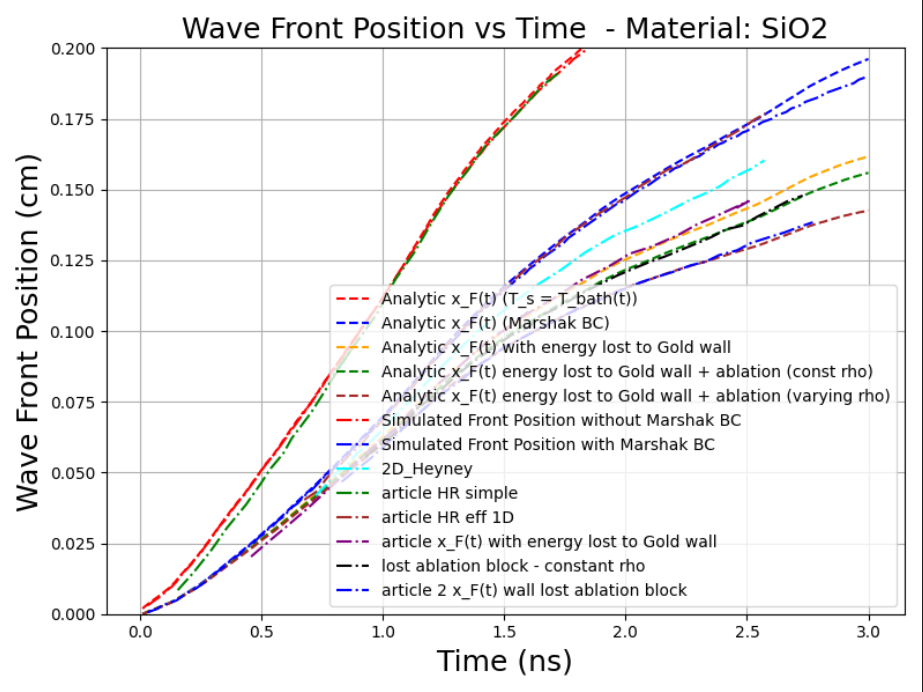
\includegraphics[width=1\textwidth]{figures_1.5D/Back_SiO2.png}
    \caption{Comparison of the front position $x_F(t)$ in the Back et al. experiment for SiO$_2$ foam between the numerical simulation, the semi-analytic models, and the digitized curves from PRR2.}
    \label{fig:Back_exp_SiO2} 
\end{figure}

\begin{figure}[h!]
    \centering
    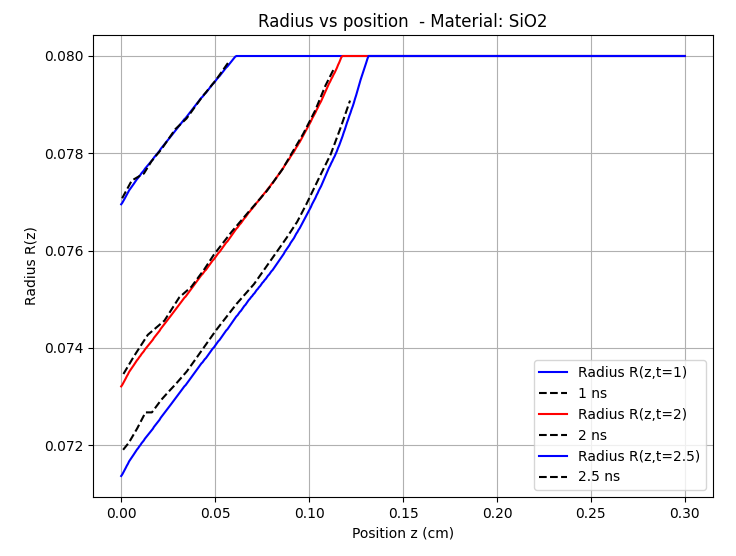
\includegraphics[width=0.7\textwidth]{figures_1.5D/Back_SiO2_radius.png}
    \caption{Comparison of the radius change due to wall ablation in the Back et al. experiment for SiO$_2$ foam between the numerical simulation and the semi-analytic models.}
    \label{fig:Back_exp_SiO2_radius_change} 
\end{figure}

\begin{figure}[h!]
    \centering
    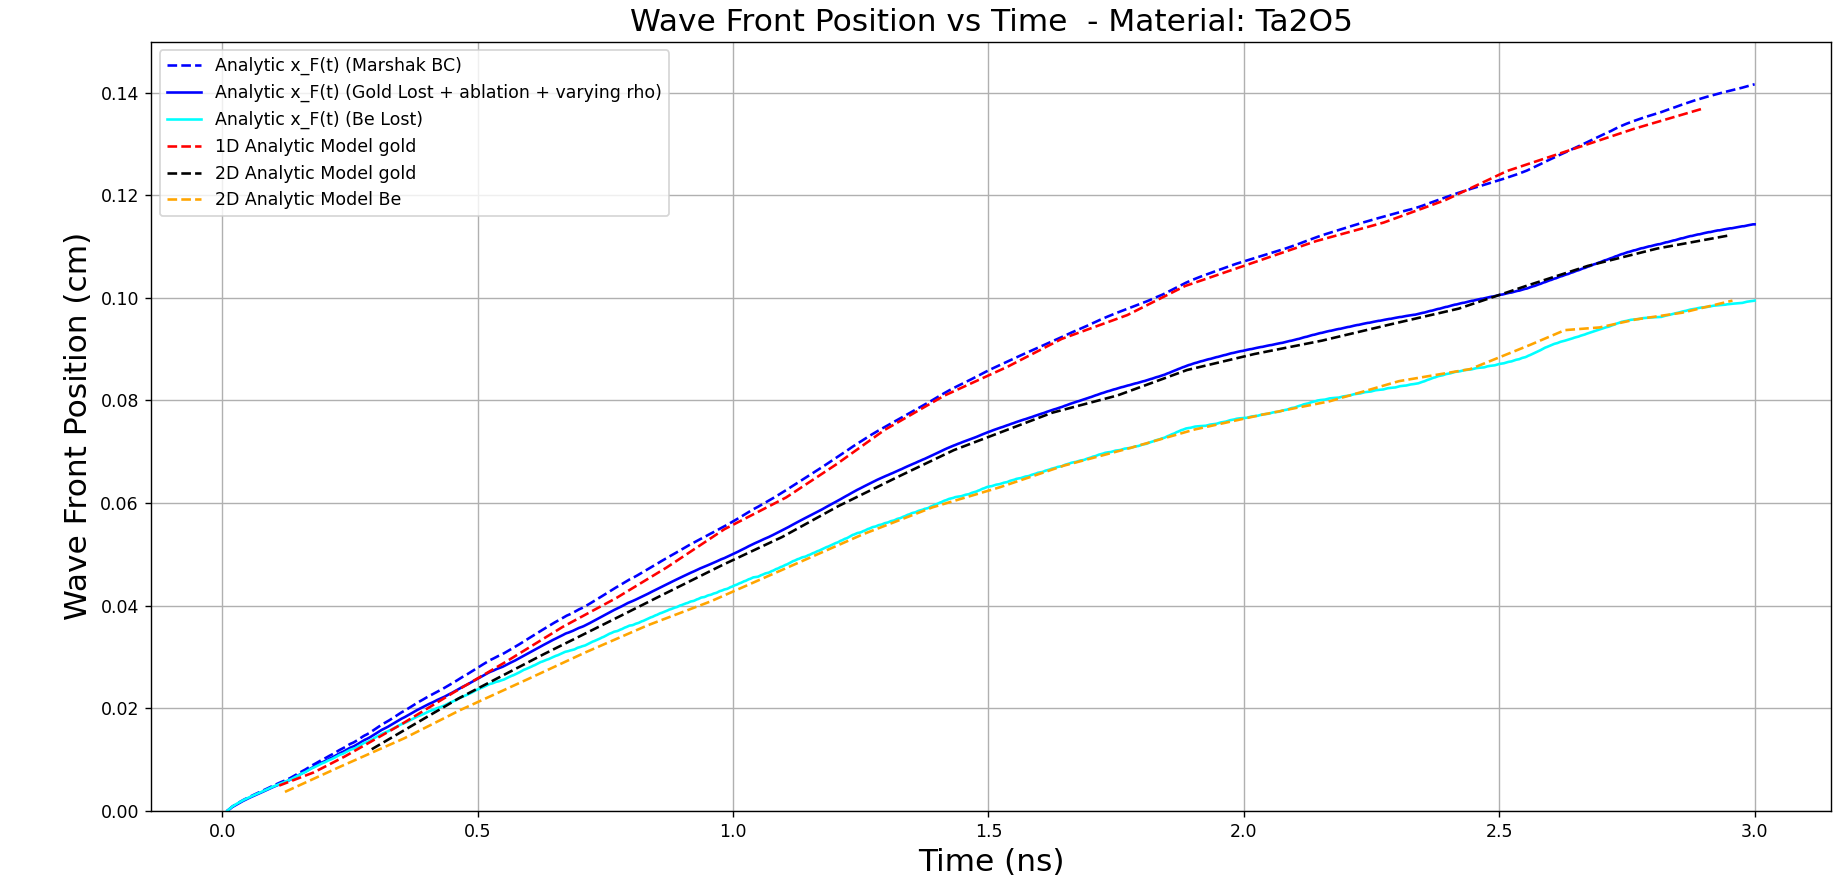
\includegraphics[width=1\textwidth]{figures_1.5D/Back_Ta2O5.png}
    \caption{Comparison of the front position $x_F(t)$ in the Back et al. experiment for Ta$_2$O$_5$ foam between the numerical simulation, the semi-analytic models, and the digitized curves from PRR2.}
    \label{fig:Back_exp_Ta2O5} 
\end{figure}

Now I'll introduce the Massen et al. experiment, which is a C$_{11}$H$_{16}$Pb$_{0.3852}$ foam with density 0.08 g/cc, several lengths (0.05 to 0.3 mm). The drive temperature is constant (100, 120, or 150~eV), and the front position is shown in Fig.~10 for the 1D (Marshak-boundary) model. See Fig.~\ref{fig:Massen_exp_Ta2O5} in this file: the late-time agreement is pretty good, but in the paper there is a strange initial offset (i.e., the curve does not start from zero).

\begin{figure}[h!]
    \centering
    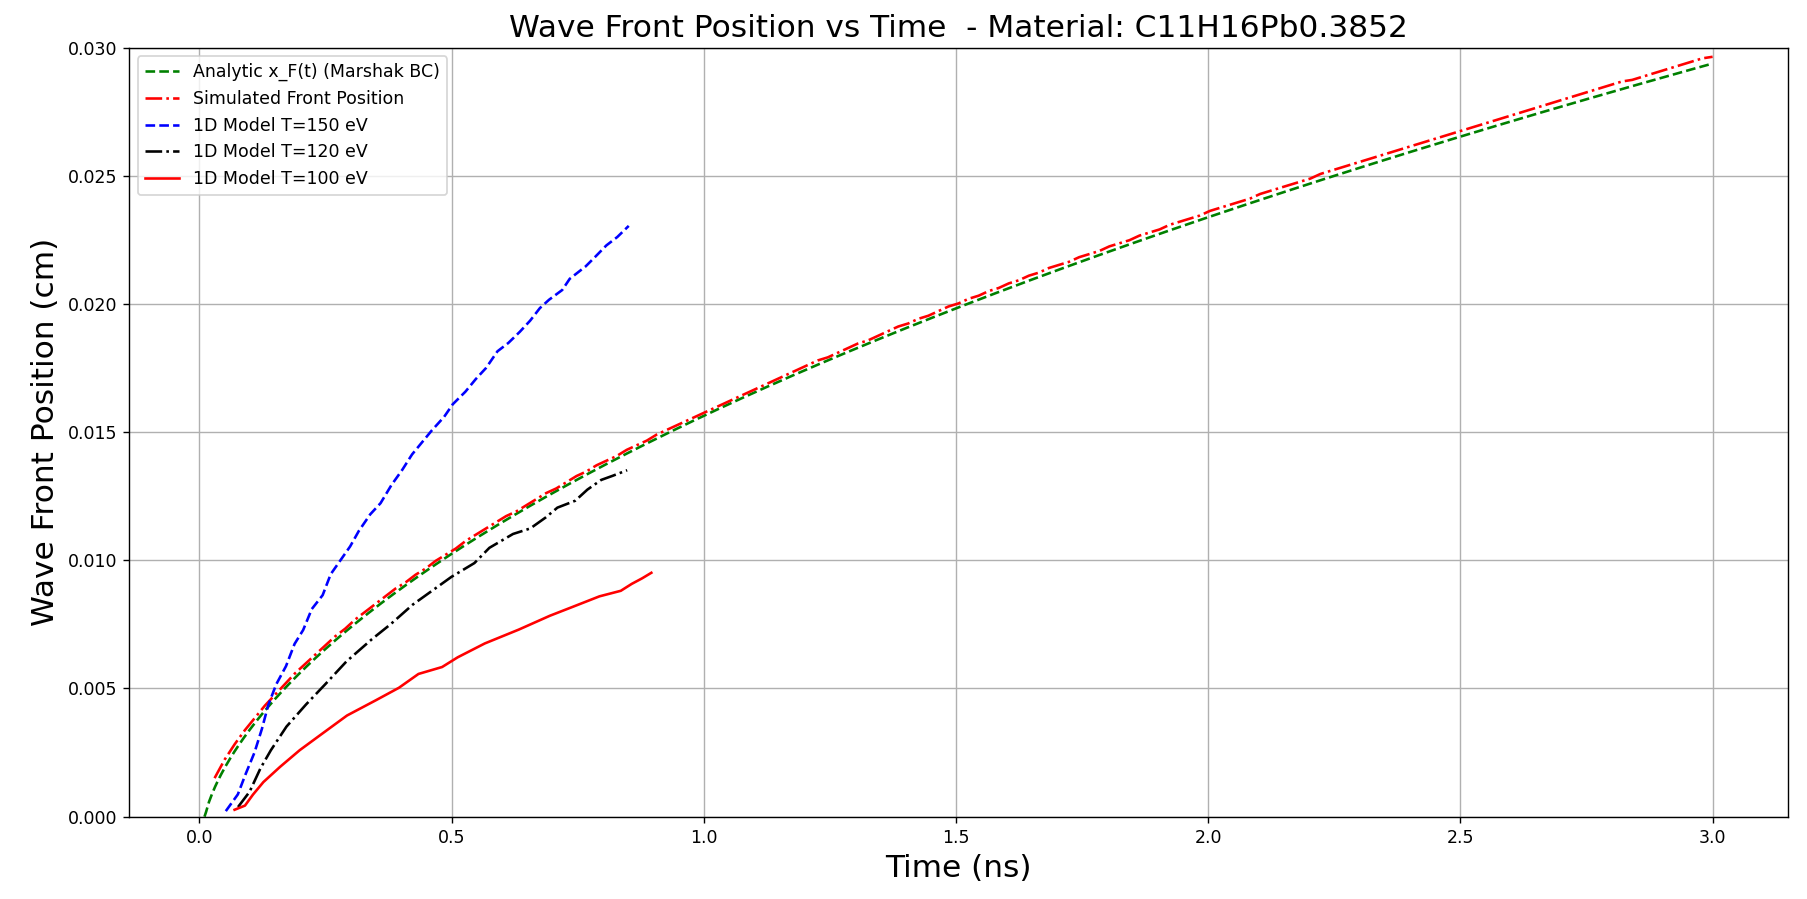
\includegraphics[width=1\textwidth]{figures_1.5D/Massen_120.png}
    \caption{Comparison of the front position $x_F(t)$ in the Massen et al. experiment (for 120~eV) for C$_{11}$H$_{16}$Pb$_{0.3852}$ foam between the numerical simulation, the semi-analytic models, and the digitized curves from PRR2.}
    \label{fig:Massen_exp_Ta2O5}
\end{figure}

Now I'll introduce the Xu et al. experiment, which is a pure CH foam and a doped C$_{15}$H$_{20}$O$_6$Pb foam with density 0.05 g/cc, length 0.3 and 0.4 mm, and diameter 0.6 mm. The drive temperature is shown in Fig.~12(b) of the paper, and the front position is shown in Fig.~12(a). In this file, Figs.~\ref{fig:Xu_exp_CH_front}--\ref{fig:Xu_exp_CHCu_front} show the comparison between the semi-analytic models and the digitized curves from PRR2.

\begin{figure}[h!]
    \centering
    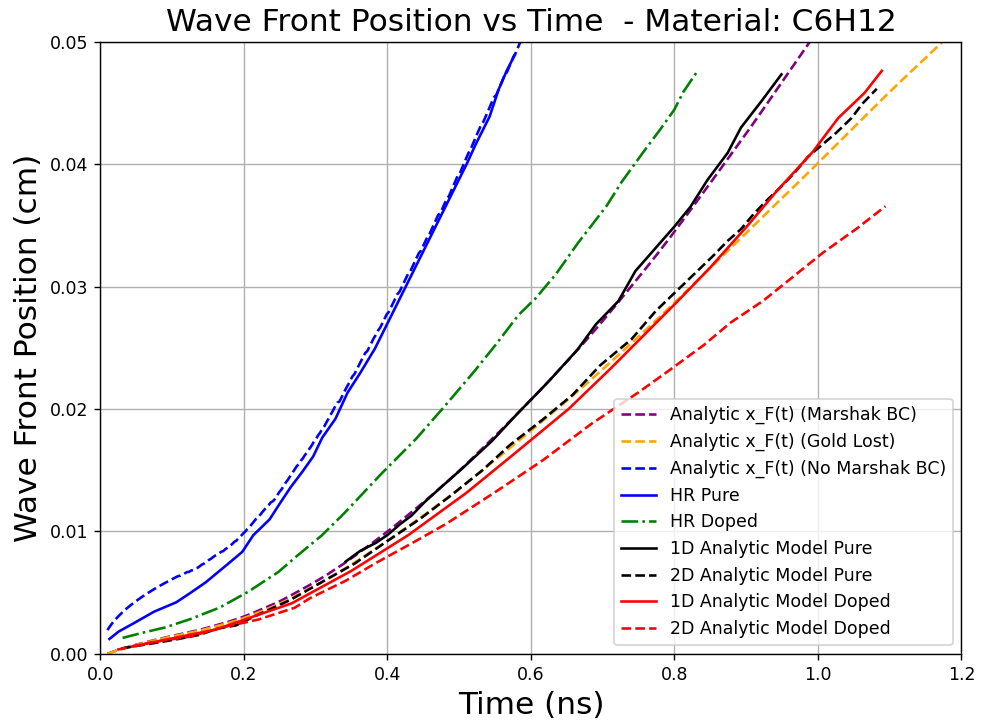
\includegraphics[width=0.75\textwidth]{figures_1.5D/Xu_C6H12_front.png}
    \caption{Comparison of the front position $x_F(t)$ in the Xu et al. experiment for pure CH foam between the semi-analytic models, and the digitized curves from PRR2.}
    \label{fig:Xu_exp_CH_front}
\end{figure}

\begin{figure}[h!]
    \centering
    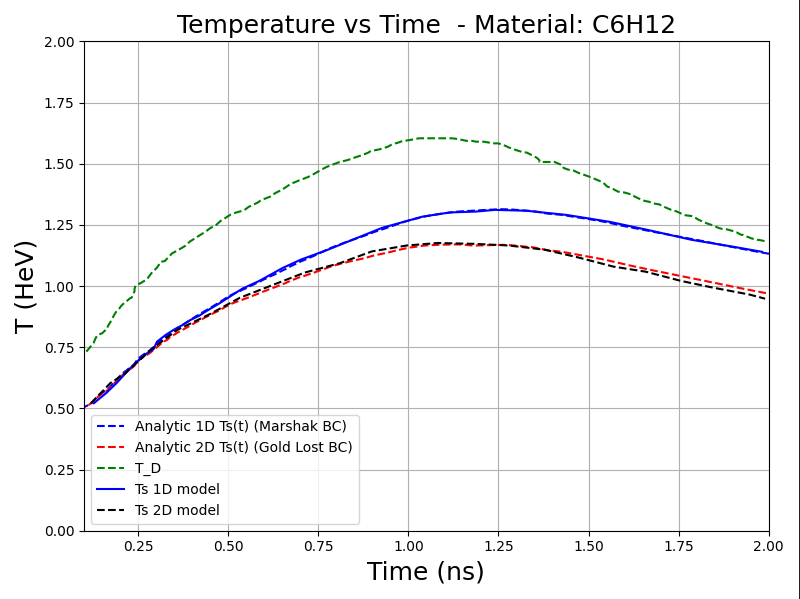
\includegraphics[width=0.75\textwidth]{figures_1.5D/Xu_C6H12_Temperature.png}
    \caption{Comparison of the surface temperature $T_S(t)$ in the Xu et al. experiment for pure CH foam between the semi-analytic models, and the digitized curves from PRR2.}
    \label{fig:Xu_exp_CH_Temperature}
\end{figure}

\begin{figure}[h!]
    \centering
    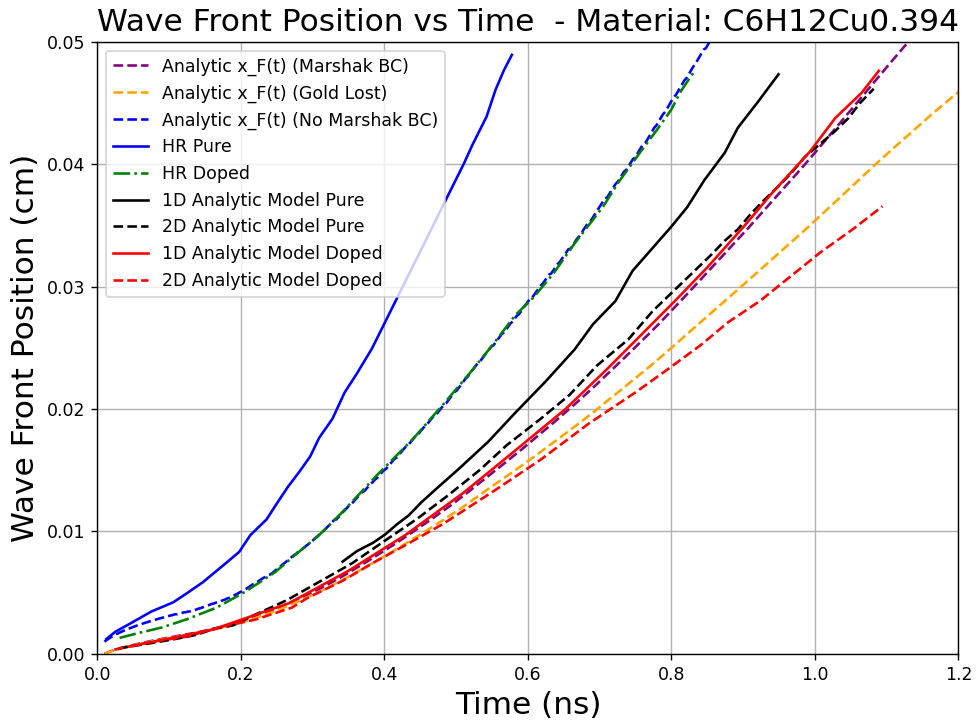
\includegraphics[width=0.75\textwidth]{figures_1.5D/Xu_C6H12Cu0.394.png}
    \caption{Comparison of the front position $x_F(t)$ in the Xu et al. experiment for doped (C$_{15}$H$_{20}$O$_6$Cu$_{0.394}$) CH foam between the semi-analytic models, and the digitized curves from PRR2.}
    \label{fig:Xu_exp_CHCu_front}
\end{figure}

Now I'll introduce the Moore et al. experiment, which is a C$_8$H$_7$Cl foam with density 0.1 g/cc, length 2.8 mm, and diameter 2 mm. The drive temperature is shown in the original experiment paper, and the front position is shown in Fig.~15(b). In Fig.~\ref{fig:Moore_exp_C8H7Cl_front}, I apply the same conditions to the semi-analytic model I coded. The fit is pretty good. The interesing thing is that the SiO2 (Fig.~15(a)) case was not as good as this one. Shay told me that there is a strange thing in the original Moore et al. paper about SiO$_2$. The Energy which was deposited to the foam is different from the energy was in the C$_8$H$_7$Cl. So, the drive temperture must be different, and beacuse $E\propto T^4$, we can scale the drive temperature for SiO$_2$ as below: 
\[
T_{D, SiO_2} (eV) = \frac{E_{SiO_2}}{E_{C_8H_7Cl}} \times T_{D, C_8H_7Cl} (eV) = \frac{340.2}{368.1} \times T_{D, C_8H_7Cl} (eV).
\]
In Fig.~\ref{fig:Moore_exp_SiO2_front}, I use this scaled drive temperature for SiO$_2$, and the fit is better than before.

\begin{figure}[h!]
    \centering
    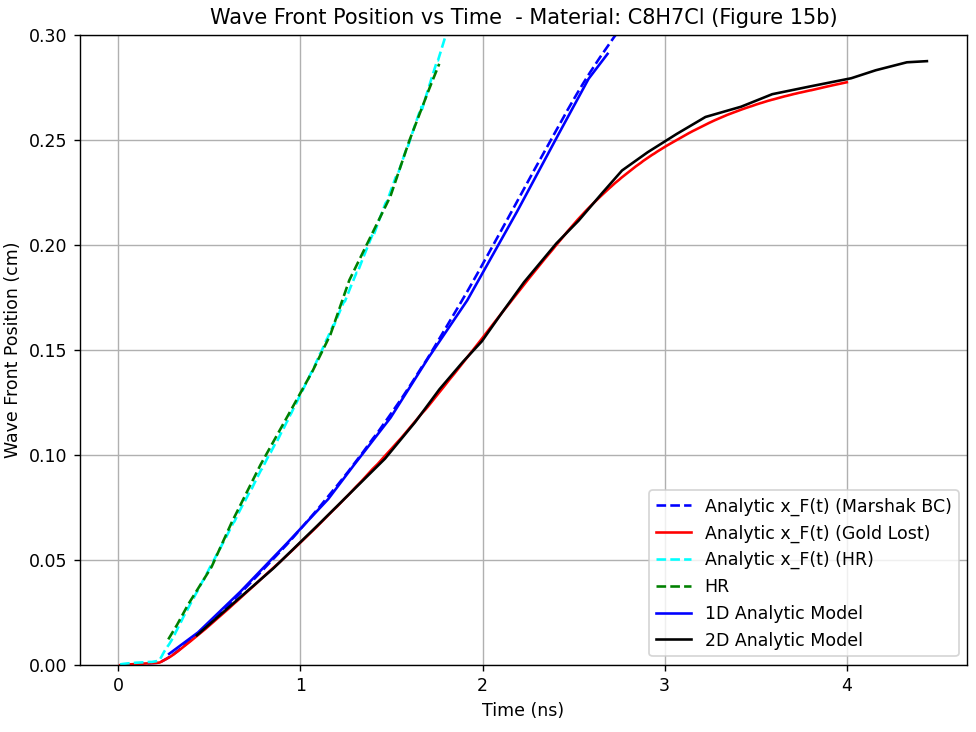
\includegraphics[width=1\textwidth]{figures_1.5D/Moore_C8H7Cl.png}
    \caption{Comparison of the front position $x_F(t)$ in the Moore et al. experiment for C$_8$H$_7$Cl foam between the semi-analytic models, and the digitized curves from PRR2.}
    \label{fig:Moore_exp_C8H7Cl_front}
\end{figure}

\begin{figure}[h!]
    \centering
    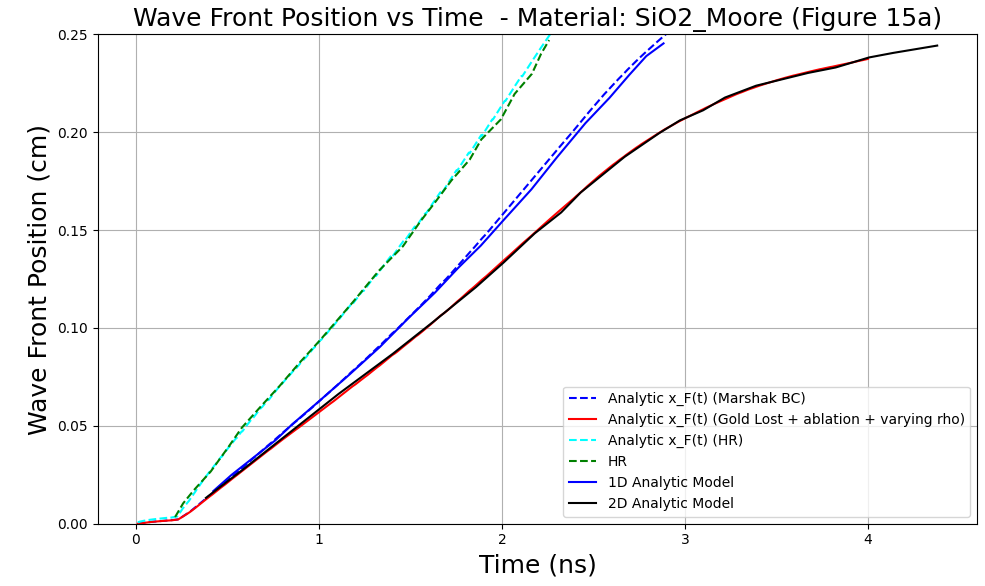
\includegraphics[width=1\textwidth]{figures_1.5D/Moore_SiO2.png}
    \caption{Comparison of the front position $x_F(t)$ in the Moore et al. experiment for SiO$_2$ foam between the semi-analytic models, and the digitized curves from PRR2. Using the scaled drive temperature for SiO$_2$ as explained in the text.}
    \label{fig:Moore_exp_SiO2_front}
\end{figure}

Now I'll introduce the Keiter et al. experiment, which includes pure and Au-doped C$_{15}$H$_{20}$O$_6$ foam with density 0.0625 (doped) and 0.065 (pure) g/cc, length 1.2 mm, and diameter 0.8 mm. The drive temperature is shown in the original experiment paper (in blue), and the front position is shown in Fig.~16. The heat front was defined as the location where the radiative flux reaches 40\% of the maximal value, so we use the formula from the paper (Eq.~(9)) with $f=0.4$ for a consistent comparison. In Fig.~\ref{fig:main} the same conditions are applied for both pure and doped foams, and we see good agreement with PRR2. The parameter that improved the fit is the $\tilde{u}$ value, which I set to 0.05302 for all densities; this is of course not strictly correct, because for each experiment $\rho$ is slightly different.

\begin{figure}[h!]
    \centering
    \begin{subfigure}{0.45\textwidth}
        \centering
        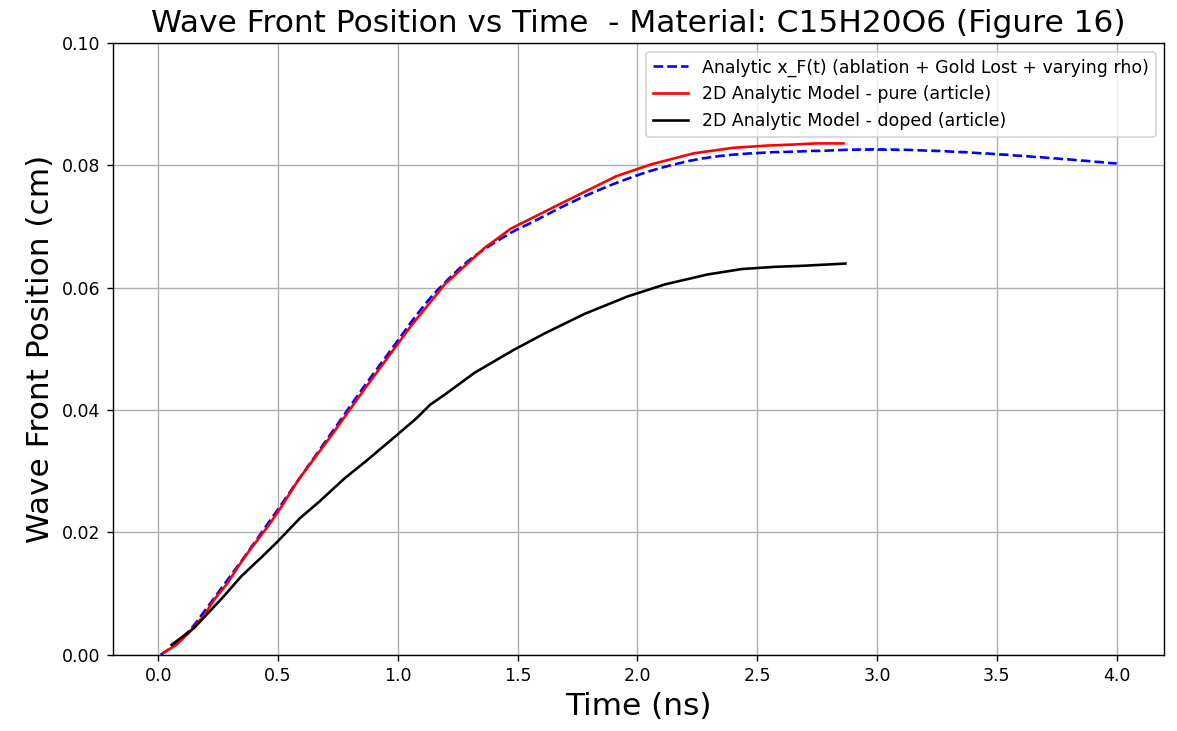
\includegraphics[width=\linewidth]{figures_1.5D/Keiter_pure.png}
        \caption{Comparison of the front position $x_F(t)$ in the Keiter et al. experiment for pure C$_{15}$H$_{20}$O$_6$ foam between the semi-analytic models, and the digitized curves from PRR2.}
        \label{fig:sub1}
    \end{subfigure}
    \hfill
    \begin{subfigure}{0.45\textwidth}
        \centering
        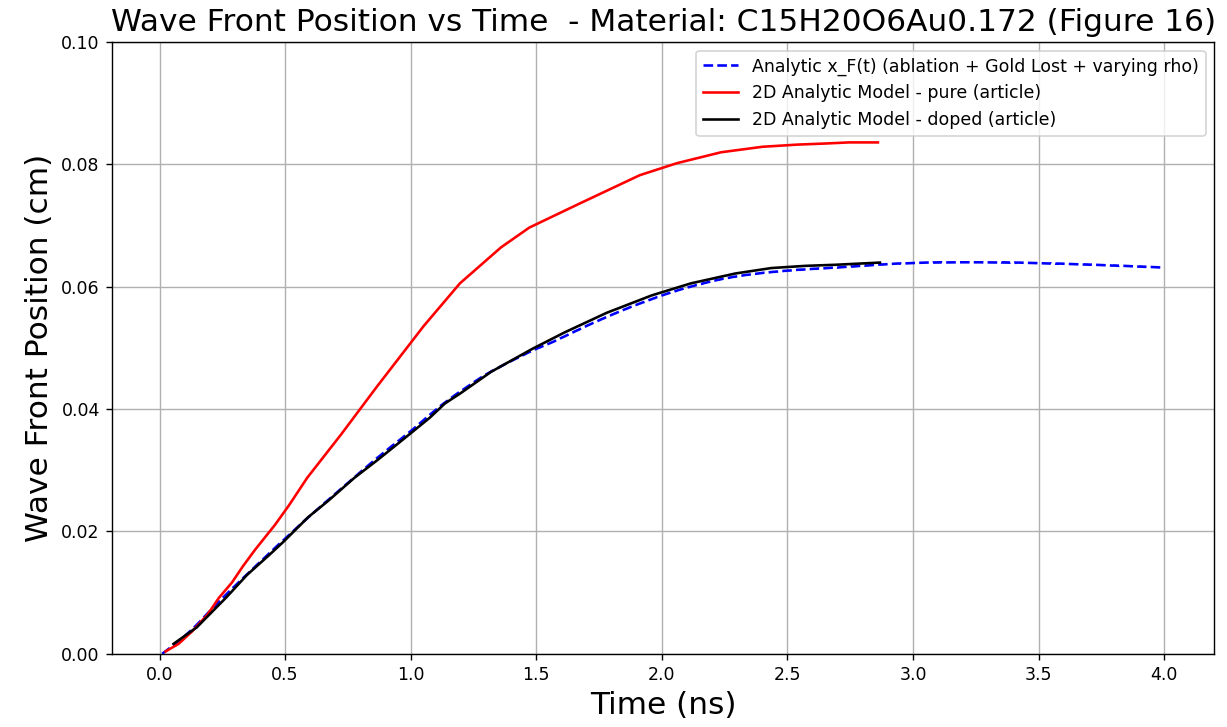
\includegraphics[width=\linewidth]{figures_1.5D/Keiter_doped.png}
        \caption{Comparison of the front position $x_F(t)$ in the Keiter et al. experiment for Au-doped C$_{15}$H$_{20}$O$_6$ foam between the semi-analytic models, and the digitized curves from PRR2.}
        \label{fig:sub2}
    \end{subfigure}
    \caption{Comparison of the front position $x_F(t)$ in the Keiter et al. experiment for Au-doped C$_{15}$H$_{20}$O$_6$ foam between the semi-analytic models, and the digitized curves from PRR2.}
    \label{fig:main}
\end{figure}

Lastly I'll introduce the Ji-Yan et al. experiment, which is a CH foam with density 0.16 g/cc, length 0.3 mm, and diameter 0.2 mm. The drive temperature is shown in the original experiment paper, and the front position is shown in Fig.~17. The heat front was defined as the location where the radiative flux reaches 50\% of the maximal value ($f=0.5$). The fit is not as good here, and it looks like I would get a better fit if $f$ were smaller than 0.5 (or even closer to 0). In Fig.~\ref{fig:Ji-Yan_exp_CH_front} the comparison is shown.

\begin{figure}[h!]
    \centering
    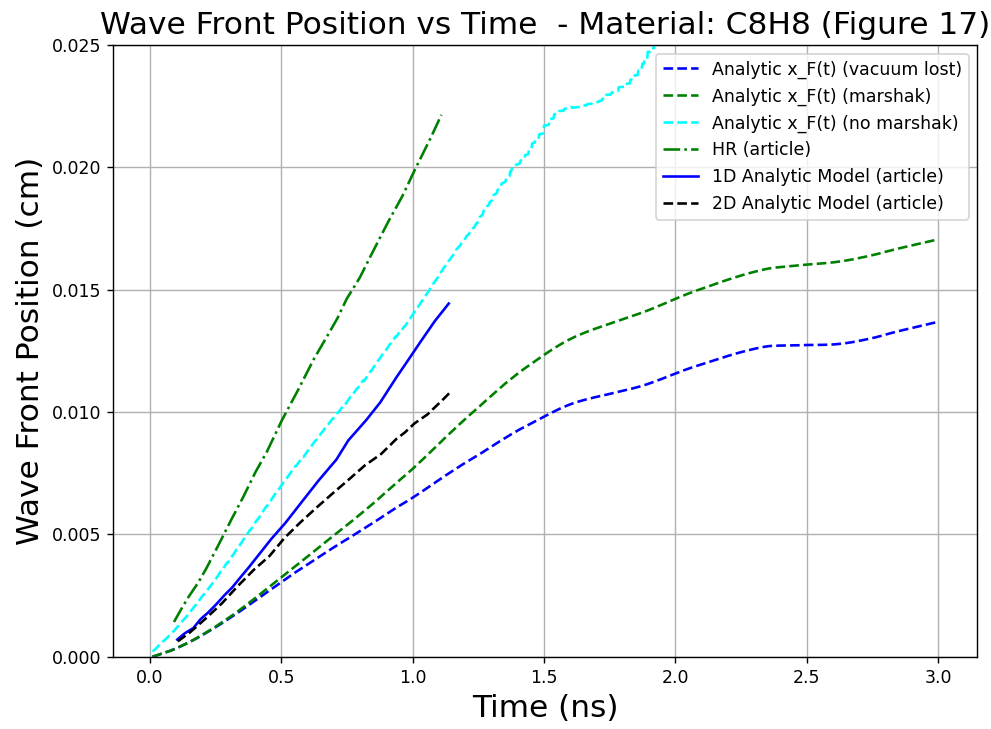
\includegraphics[width=1\textwidth]{figures_1.5D/Ji-Yan_exp.png}
    \caption{Comparison of the front position $x_F(t)$ in the Ji-Yan et al. experiment for pure CH foam between the numerical simulation, the semi-analytic models, and the digitized curves from PRR2.}
    \label{fig:Ji-Yan_exp_CH_front}
\end{figure}

\end{document}